\documentclass[10pt]{beamer}
\setbeamertemplate{navigation symbols}{}

\setbeamercolor{frametitle}{fg=black,bg=red}
\setbeamercolor{title}{fg=black,bg=white!85!orange}
\usetheme{CambridgeUS}

\usepackage[russian]{babel}
\usepackage[utf8]{inputenc}
\usepackage{listingsutf8}
\usepackage{algorithm}
\usepackage{algpseudocode}
\usepackage{tcolorbox}

\usepackage{array}
\usepackage{multirow}

\lstloadlanguages{[Auto]Lisp}

\lstdefinestyle{base_listing}{
  extendedchars     = {true},
  inputencoding     = {utf8}, 
  basicstyle        = {\ttfamily \scriptsize},
  keywordstyle      = {\rmfamily \bfseries},
  commentstyle      = {\rmfamily \itshape},
  tabsize           = {2},
  flexiblecolumns   = {false},
  showstringspaces  = {falsedany},
  breaklines        = {true}, 
  breakatwhitespace = {true}
}

\definecolor{lred}{rgb}{1,0.78,0.79}
\definecolor{lgreen}{rgb}{0.9,1,0.8}


\lstdefinestyle{base_listing_floating}{
  style   = {base_listing},
  numbers = {none},
  % float = {h}, % float right where we put it
  % aboveskip = 0pt, 
  % belowskip = 0pt
}


\lstdefinestyle{crs_cpp}{
  style    = {base_listing},
  language = {C++}
}


% очень бедное определение ассемблера LLVM для листингов
% выделены только ключевые слова, встречающиеся в примерах
\lstdefinelanguage{LLVM-asm}
{
  morekeywords = {
    load, store, malloc, alloca, free, getelementptr,
    add, sub, insertvalue, extractvalue, icmp, call
  },
  sensitive   = false,
  morecomment = [l]{;}
}

\lstdefinestyle{crs_llvm}{
  style    = {base_listing_floating},
  language = {LLVM-asm}
}



\beamersetuncovermixins{\opaqueness<1>{25}}{\opaqueness<2->{15}}
\begin{document}
\title[Scheduler]{Разработка и встраивание планировщика в ОС Linux}
\author[Степанов Даниил]{Студент: Степанов Даниил}
\institute[]{Санкт-Петербургский политехнический университет Петра Великого}
\date{\today} 


\begin{frame}
\titlepage
\end{frame}

%\begin{frame}\frametitle{Table of contents}\tableofcontents
%\end{frame} 


\begin{frame}\frametitle{Планирование}
Дисциплина планирования должна быть:
\begin{itemize}
\item справедливой
\item обеспечивать максимальную пропускную способность системы
\item приемлемые времена ответа для максимального количества пользователей, работающих в интерактивном режиме
\item предсказуемость
\item минимальные накладные расходы
\item ...
\end{itemize}
\end{frame}

\begin{frame}\frametitle{Факторы, учитываемые при планировании}
Для реализации перечисленных целей механизмы планирования должны учитывать следующие факторы:
\begin{itemize}
\item лимитируется ли процесс вводом-выводом или ЦП
\item является ли процесс пакетным или диалоговым
\item обязательно ли малое время ответа
\item приоритет каждого процесса
\item частоту переключений с низкоприоритетных процессов, ожидающих освобождения уже занятых ресурсов
\item длительность периода времени, в течение которого ожидает каждый процесс
\item суммарное время работы каждого процесса и оценочное время, необходимое каждому процессу для завершения
\end{itemize}
\end{frame}

\begin{frame}\frametitle{Переключение}
Планирование без переключения предусматривает, что после предоставления ресурсов ЦП какому-либо процессу, отобрать ЦП у этого процесса нельзя. \\ \ \\
Если же ресурсы ЦП можно отобрать, то говорят о планировании с переключением.
\end{frame}

\begin{frame}\frametitle{Приоритеты}
\begin{itemize}
\item Система может присваивать процессам приоритеты автоматически или они могут назначаться извне \item Приоритеты могут быть заслуженными или купленными. Они могут быть статическими или динамическими
\item Они могут назначаться по какому-то рациональному принципу или присваиваться в ситуациях, когда системе просто необходимо каким-либо образом различать процессы
\end{itemize}
\end{frame}

\begin{frame}\frametitle{Планировщик О(1)}
\center
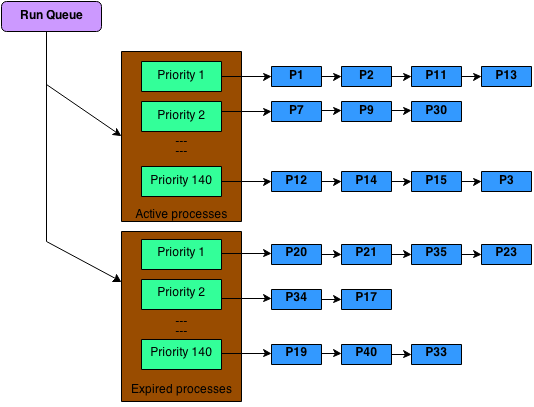
\includegraphics[width=10cm, height=10cm,keepaspectratio]{sched4}
\end{frame}

\begin{frame}\frametitle{Completely Fair Scheduler}
\center
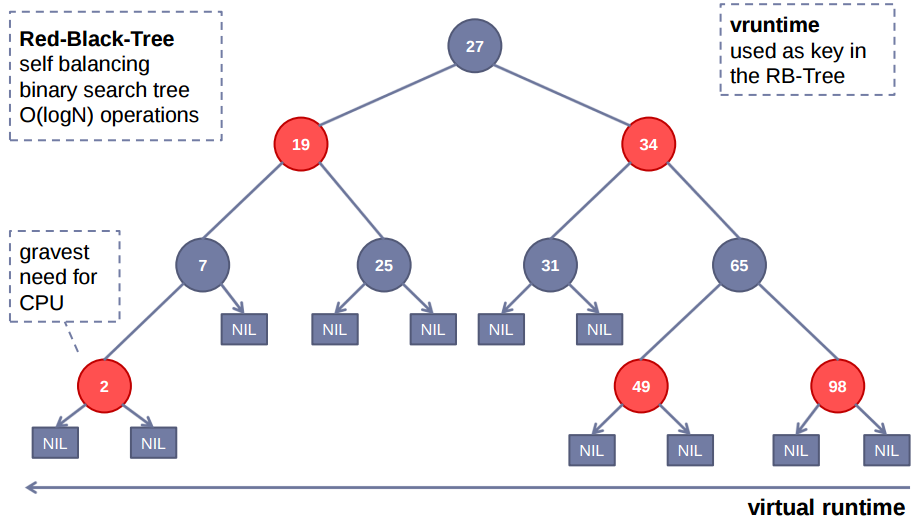
\includegraphics[width=10cm, height=10cm,keepaspectratio]{sched5}
\end{frame}

\begin{frame}\frametitle{Earliest deadline first}
\center
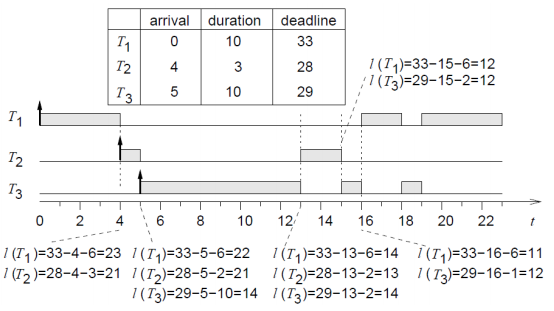
\includegraphics[width=10cm, height=10cm,keepaspectratio]{sched6}
\end{frame}

\begin{frame}[fragile]
\begin{lstlisting}
user@debian:~$ uname -r
3.16.0-4-586
user@debian:~$ dmesg | grep scheduler
[    0.642934] io scheduler noop registered
[    0.642937] io scheduler deadline registered
[    0.642959] io scheduler cfq registered (default)
user@debian:~$ cat /sys/block/sda/queue/scheduler 
noop deadline [cfq] 
root@debian:echo deadline >/sys/block/sda/queue/scheduler
user@debian:~$ cat /sys/block/sda/queue/scheduler 
noop [deadline] cfq 
\end{lstlisting}
\end{frame}

\begin{frame}\frametitle{Встраивание своего планировщика}
\begin{itemize}
\item /usr/src/linux-*/kernel/sched.c
\item sudo apt-get install linux-source-2.6.24 kernel-package libncurses5-dev fakeroot 
\item tar xvf linux-source-2.6.24.tar
\item cp /boot/config-`uname -r` /usr/src/linux/.config
\item fakeroot make-kpkg --initrd --append-to-version=-custom kernel\_image kernel\_headers 
\item dpkg -i linux-image-2.6.24.3-custom\_2.6.24.3-custom-10.00.Custom\_i386.deb
\end{itemize}
В текущей версии ядра команды не изменились
\end{frame}

\begin{frame}\frametitle{Основные функции}
\center
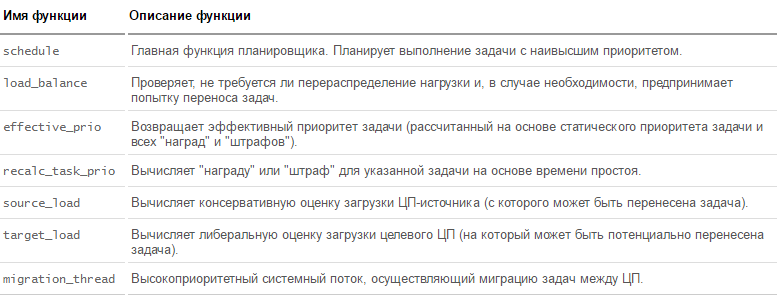
\includegraphics[width=12cm, height=12cm,keepaspectratio]{sched7}
\end{frame}

\begin{frame}
Задания на курсовую работу:
\begin{itemize}
\item Разработать планировщик О(1) и встроить его в ядро
\item На собственных тестах сравнить производительность встроенных и разработанного планировщиков
\end{itemize}
\end{frame}

\end{document}